
\section*{Tarea 2}

\textbf{1. Absorción de cloro en una película descendente}\textit{(Problema. 18A.4, Bird et al.)}
\flushleft
\begin{minipage}{0.3\textwidth} % Tamaño del bloque de la imagen
    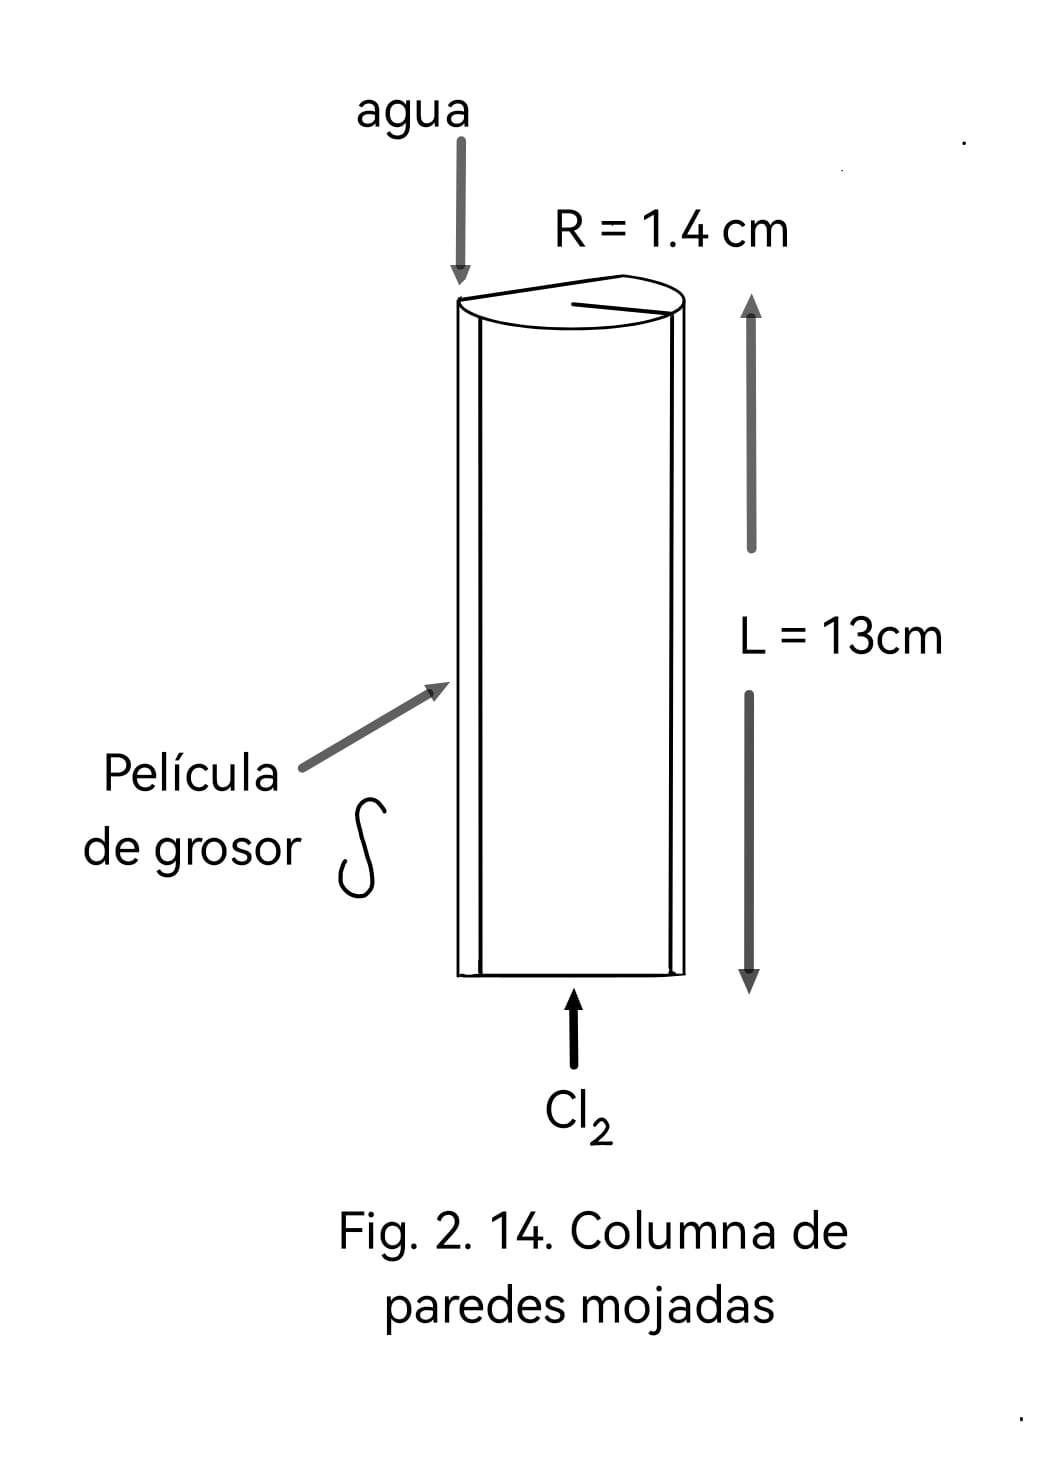
\includegraphics[width=\linewidth]{imagen.1.jpg} % Imagen ajustada al bloque
\end{minipage}
\hfill % Espaciado entre imagen y texto
\begin{minipage}{0.65\textwidth} % Tamaño del bloque del texto
Cloro gaseoso se absorbe en agua de la columna de la Fig. 2.14. La velocidad del agua es 17.7 cm/s. La difusividad en la fase líquida del sistema Cl$_2$-H$_2$O es de $1.26 \times 10^{-5}$ cm$^2$/s y la concentración de saturación es de 0.823 g Cl$_2$/100 g H$_2$O. ¿Cuál es la velocidad de absorción en mol/hr?
\vspace{0.5cm} % Espacio antes de la respuesta 
\flushleft
\textbf{Respuesta:} \quad 0.273 \text{ gmol/hr}
\end{minipage}
\vspace{0.5cm} 

\textbf{2.Método para separar helio del gas natural} \textit{(Problema. 18.B.8, Bird et al.)}
\flushleft
\vspace{0.4cm}
\begin{minipage}{0.4\textwidth} % Tamaño del bloque de la imagen
    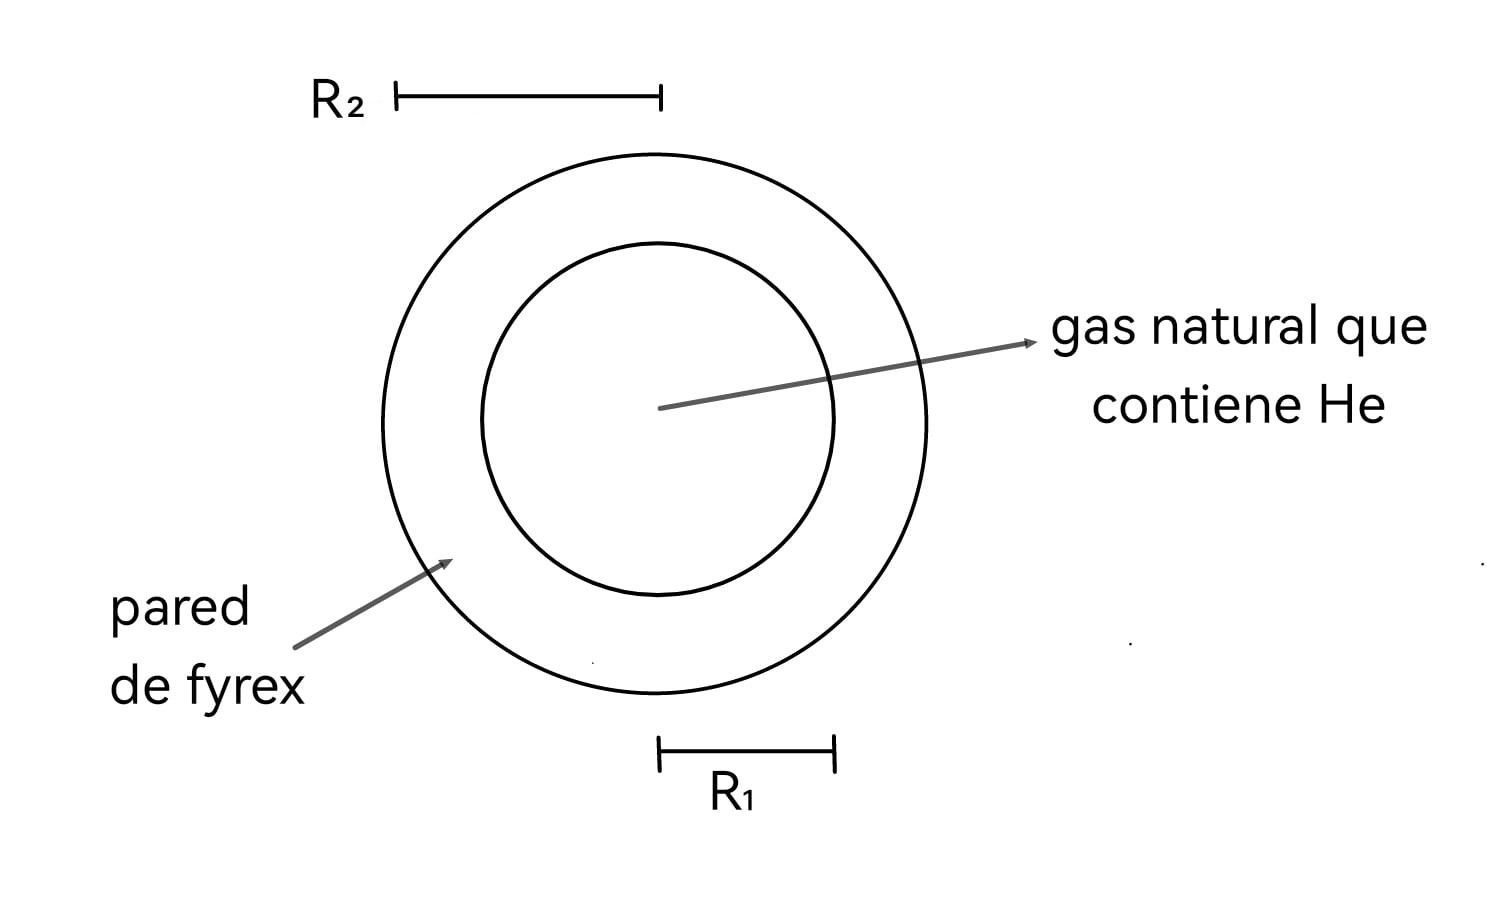
\includegraphics[width=\linewidth]{imagen.2.jpg} % Imagen ajustada al bloque
\end{minipage}
\hfill % Espaciado entre imagen y texto
\begin{minipage}{0.55\textwidth} % Tamaño del bloque del texto
La pared de vidrio Pyrex es permeable solamente al He.Suponga que el He está contenido en el recipiente. Obtenga una expresión de la difusión del He a través de la pared, las concentraciones interfaciales del He en las paredes y las dimensiones del tubo.
\vspace{0.5cm} % Espacio antes de la respuesta 
\flushleft
\textbf{Respuesta:
\[
W_{He} = \frac{2\pi L D_{He} (C_{He_{1}} - C_{He_{2}})}{\ln (R_2/R_1)}
\]}
\end{minipage}
\vspace{0.5cm}

\flushleft
\textbf{3. Velocidad de lixiviación} \textit{(Problema. 18.B.9, Bird et al.)}
\flushleft
\begin{minipage}{0.4\textwidth} % Tamaño del bloque de la imagen
    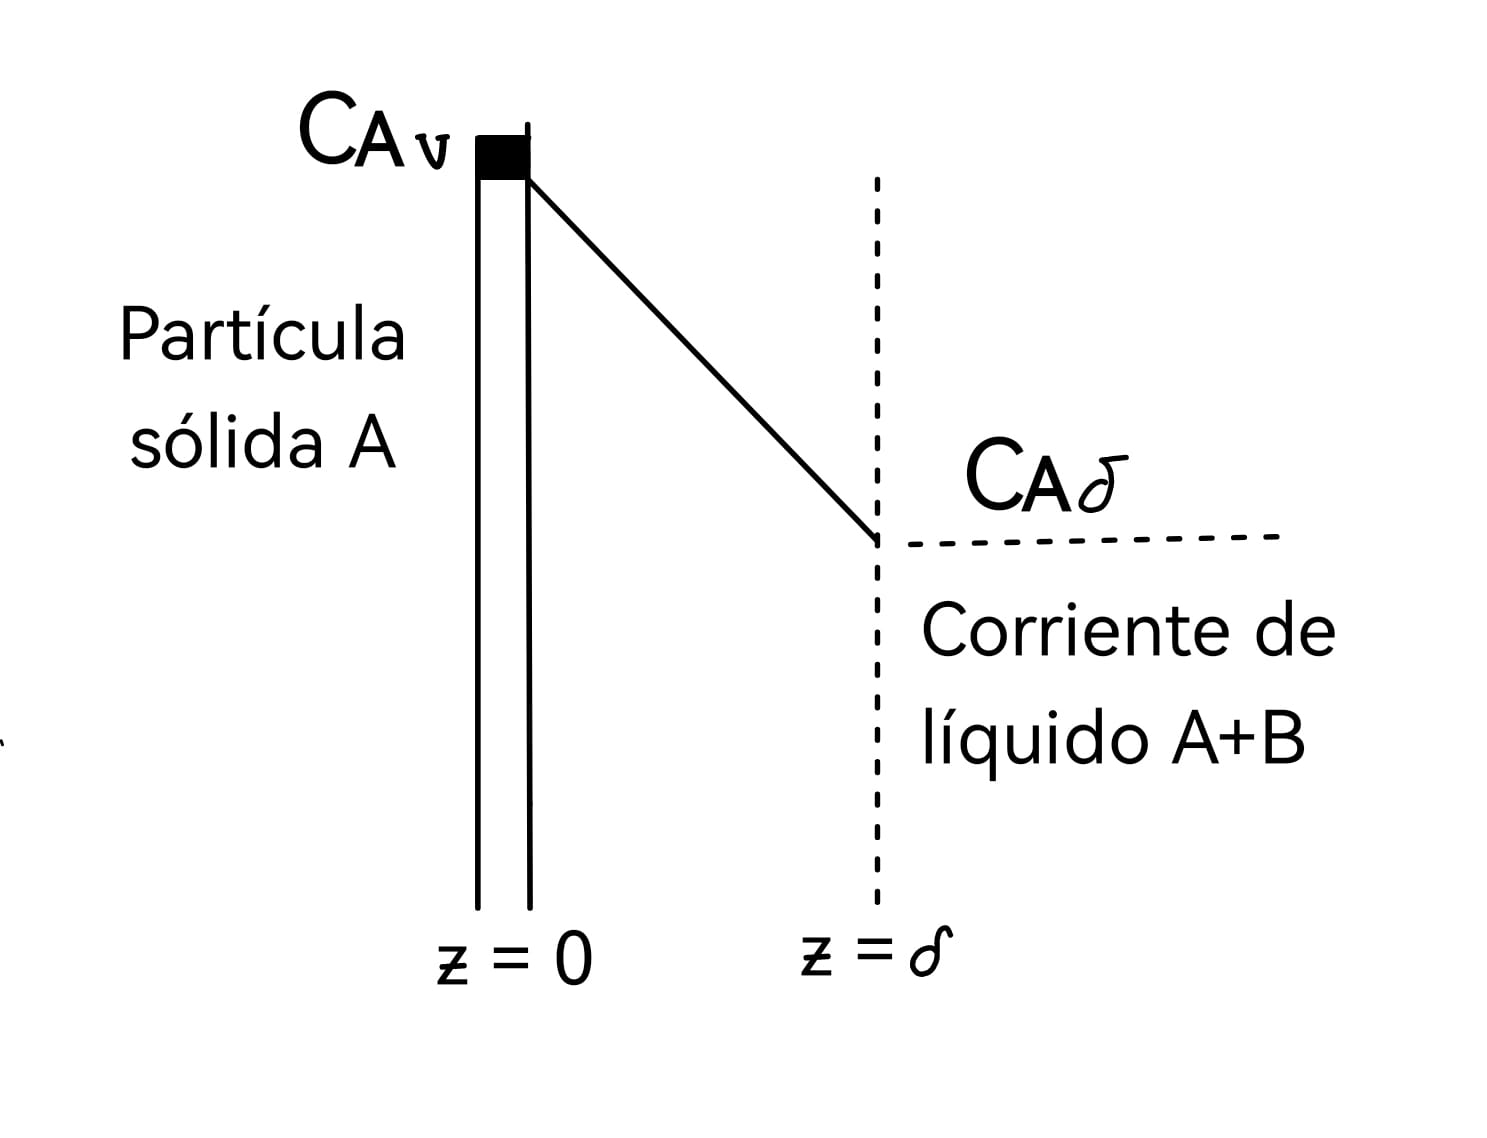
\includegraphics[width=\linewidth]{imagen.3.jpg} % Imagen ajustada al bloque
\end{minipage}
\hfill % Espaciado entre imagen y texto
\begin{minipage}{0.5\textwidth} % Tamaño del bloque del texto
La solubilidad de A en B en C$_Au$, y su concentración en B en C$_{A\delta}$. En este proceso, A difunde en B a través de una película de grosor $\delta$. Muestra que al perfil de concentraciones en lineal y que la velocidad de lixiviación es: \[N_{Au}= \frac{D_{AB}}{C_{Au}-C_{A\delta}}\]
\end{minipage}
\vspace{0.1cm} % Espacio antes de la respuesta 
\flushleft
\newpage
\textbf{4. Determinación de la difusividad del sistema éter-aire.}\textit{(Problema. 18.A.6 Birt et al)}
\vspace{0.2cm}
\flushleft
Datos de la evaporación del etil-éter con densidad del líquido de $0.7132 \text{ g/cm}^3$. El tubo tiene $6.16 \text{ mm}$ de diámetro y presión total de $747 \text{ mmHg}$  a $22^\circ C$. El peso molecular del éter $74$  y la presión de vapor a $22^\circ C$ en $498 \text{ mmHg}$. (Véase Fig. 2.1)
\vspace{0.2cm}
\flushleft
a)- Suponer un promedio de las longitudes de $Z_2 - Z_1$ para encontrar $D_{AB}$ a $747 \text{ mmHg}$ y $22^\circ C$ a partir de los datos de evaporación.
\flushleft
b)- Utilizar la ecuación $(1.53)$ para convertir los resultantes a $0^\circ C$ y $760\text{ mmHg}$ .

\begin{center}
\begin{tabular}{|c|c|}
    \hline
    \textbf{Nivel del éter (mm) medido donde el punto superior} & \textbf{Tiempo (s) para alcanzar el nivel del éter} \\
    \hline
    9-11  & 590  \\
    14-16 & 845  \\
    19-21 & 1185 \\
    24-26 & 1480 \\
    34-34 & 2055 \\
    41-46 & 2655 \\
    \hline
\end{tabular}
\end{center}

\textbf{Respuesta:} \[
D_{AB} = 0.0786 \quad \text{cm}^2/\text{s} \quad \text{a} \quad 0^\circ C \quad \text{y} \quad 760 \text{ mmHg}
\]
\newpage
\section*{Tarea 3}
\vspace{0.3cm} % Espacio antes de la respuesta 
\flushleft
\textbf{1. Mediciones de difusividad por el Método de fuente puntual.}\textit{(Problema. 18.A.5 Birt et al.)}
\vspace{0.1cm} % Espacio antes de la respuesta 
\flushleft
Una corriente de líquido B se dirige en dirección vertical, y la composición del gas se mide en varias posiciones. Calcular el gasto molar $W_A$ (g-mol/s) requerido para producir $X_A = 0.01$ en el punto 1 cm abajo de la fuente a 1 atm y $800^\circ$C, si $V_0 = 50$ cm/s y $D_{AB} = 5$ cm\textsuperscript{2}/s. 
\vspace{0.1cm} % Espacio antes de la respuesta 
\flushleft
Utilizar los resultados del \textbf{Apéndice A}.\\
\flushleft
\textbf{2. Experimentos para medir la difusividad de gases en un aparato de dos recipientes} \textit{(Prob. 18.B.6. Bird et al.)} 
\flushleft
\begin{minipage}{0.5\textwidth} % Tamaño del bloque de la imagen
    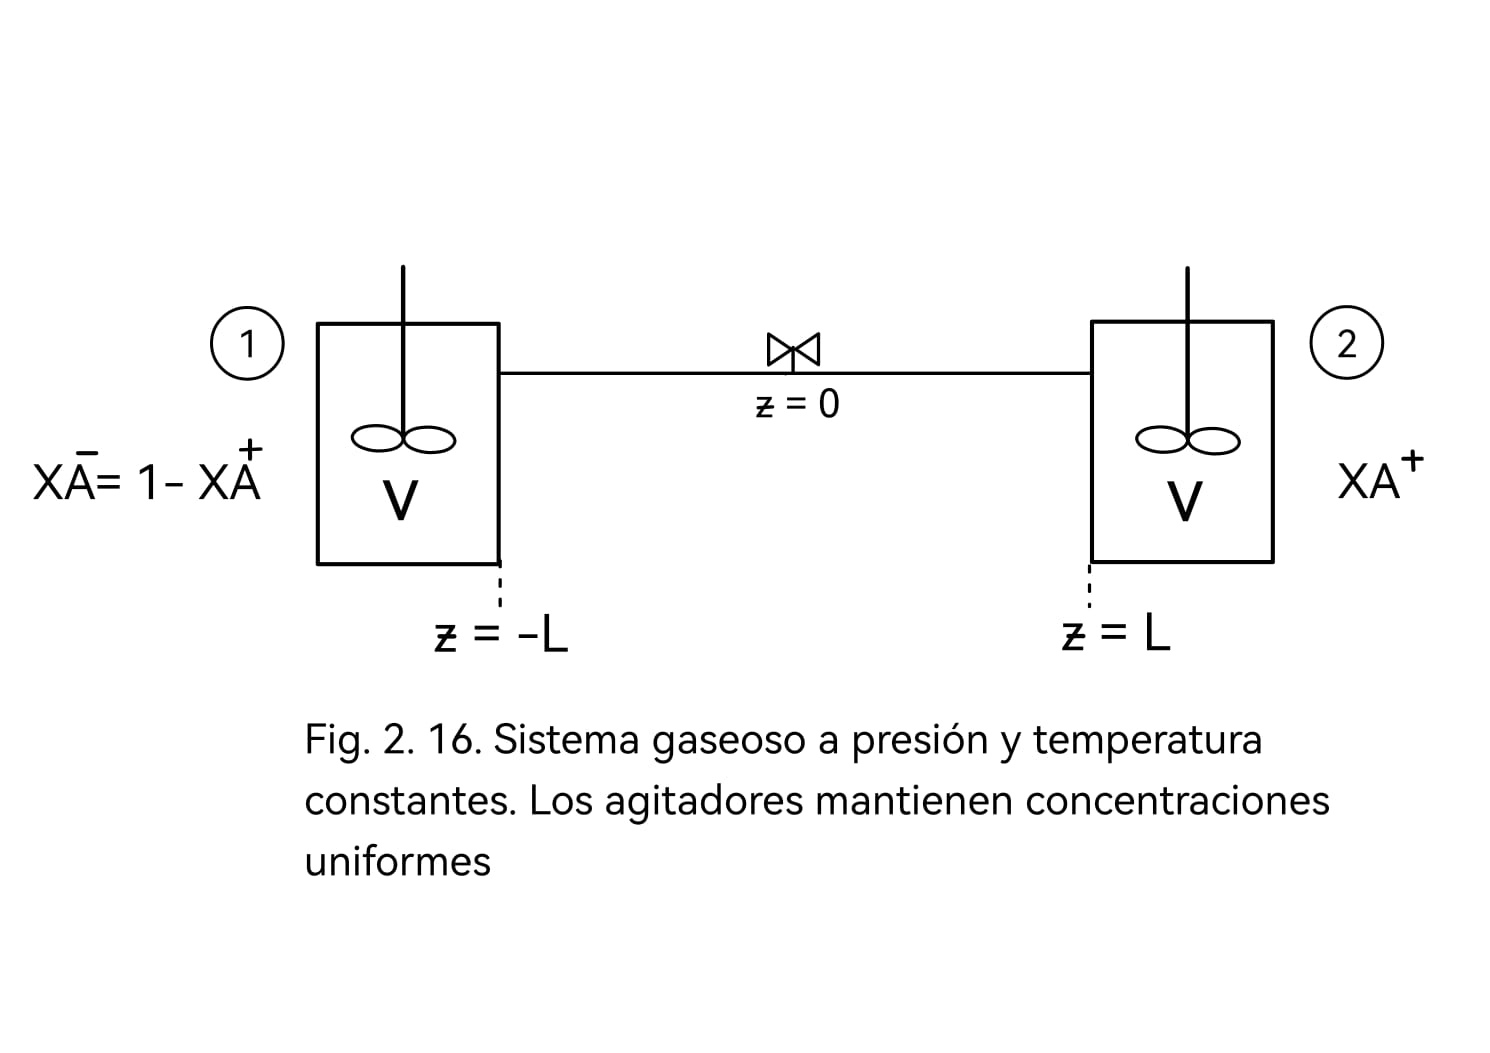
\includegraphics[width=\linewidth]{imagen.4.jpg} % Imagen ajustada al bloque
\end{minipage}
\hfill % Espaciado entre imagen y texto
\begin{minipage}{0.45\textwidth} % Tamaño del bloque del texto
El aparato tiene un gas A en el recipiente \textbf{1} y un gas B en el recipiente \textbf{2}.  La válvula se abre y la difusión comienza.  Se mide $x_A$ en función del tiempo, lo que permite medir $D_{AB}$.
\end{minipage}

\textbf{Las condiciones de frontera son:} \quad
$
x_A \bigg|_{Z=-L}= x_A^- \quad \ y \quad x_A \bigg|_{Z=L}= x_A^+ \quad
$

\textbf{Calcular lo siguiente}
\flushleft
(a)- Mostrar que $N_A$ es constante.
\flushleft
(b)- Mostrar que el flujo de masa es:\quad $ N_{A Z}= - c D_{AB} \frac{dx_A}{dz} $
\flushleft
(c)- Integrar la ecuación.
\flushleft
(d)- Evaluar la constante de integración.
\flushleft
(e)- Obtener:\quad 
$ N_{AZ} = \frac{(\frac{1}{2}-x_A^+)cD_{AB}} {L}$
\flushleft
(f)- Hacer un balance de masa en el recipiente 2 para obtener:\quad 
   $ S(\frac{1}{2}-x_A^+)\frac{cD_{AB}} {L} = V_c 
   \frac{dx_A^+}{dt} $
\flushleft
(g)- Integrar la ecuaciónpara obtener: \quad
$
\ln (\frac{\frac{1}{2}-x_A^+}{\frac{1}{2}})=\frac{-SD_{AB}t}{LV}
$
\flushleft
(h)- Hacer una gráfica para obtener $D_{AB}$ 
\vspace{0.2cm}
\newpage
\textbf{3. Difusión desde una gota suspendída.} \textit{(Problema. 18.B.7. Bird et al.)}
\flushleft
\begin{minipage}{0.45\textwidth} % Tamaño del bloque de la imagen
    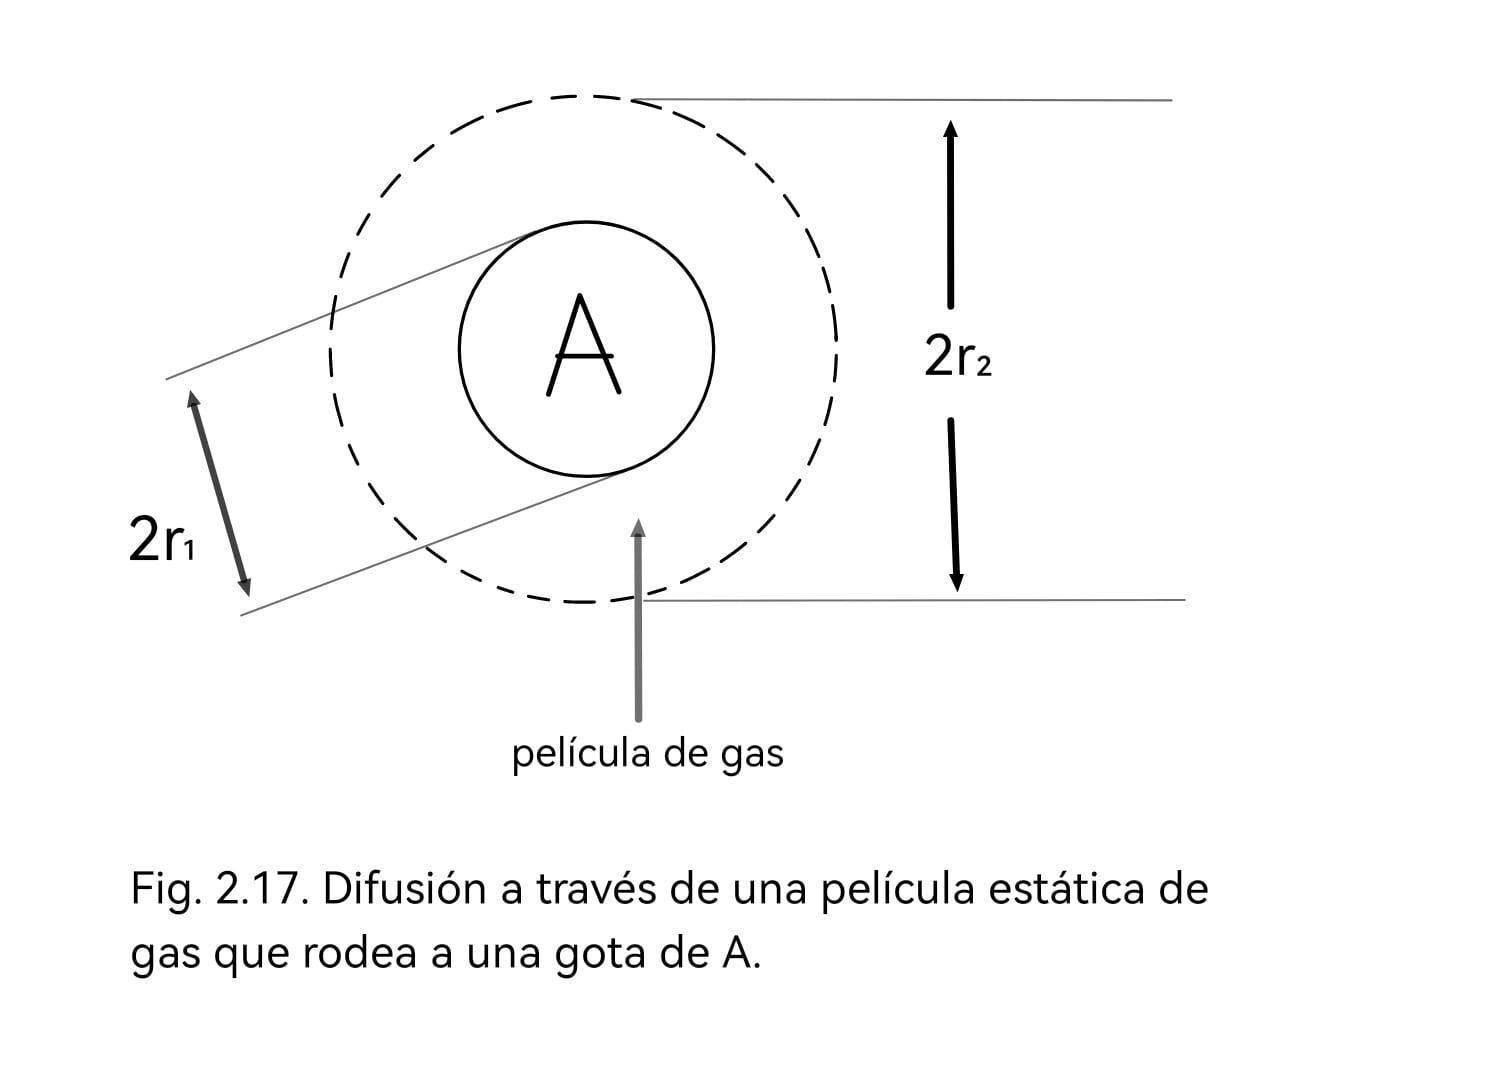
\includegraphics[width=\linewidth]{imagen.6.jpg} % Imagen ajustada al bloque
\end{minipage}
\hfill % Espaciado entre imagen y texto
\begin{minipage}{0.5\textwidth} % Tamaño del bloque del texto
Una gota de líquido A de radio $r_1$ está suspendída en una corriente de gas B. Supóngase la presencia de una película alredesor de la gota de radio $r_2$. La concentración de A en la fase gas en $x_A$, en r=$r_1$ y $x_A2$ en r=$r_2$.
\end{minipage}
Demuestra:
\flushleft
(a)- Que $r^{2}N_Ar$ es constante ene la fase gas.Evaluar la constante en r=$r_1$ para obtener $r^{2}_1N_Ar$, en la superficie de la gota:
\flushleft
(b)- La ecuacíon (1.25) y el resultado anterior resulta en: \[r^{2}_1N_Ar_1=\frac{-cD_{AB}}{1-x_A}r^{2}\frac{dx_A}{dr}\]
(c)- La integración entra $r_1$ y $r_2$ resulta en:
\[ N_{Ar_1}=\frac{cD_{AB}}{r_2-r_A1}(\frac{r_2}{r_1}){\ln {\frac{x_{B2}}{x_{B1}}}}\]
(d) Obtener el límite de esta ecuacíon cuando $r_2\rightarrow \infty$.
\newpage
\section*{Tarea 4}

\textbf{1. Absorción de cloro en ciclohexeno.} \textit{(Problema. 18.B.5 Birt et al.)}
\flushleft
El cloro se puede absorber de una mezcla Cl$_2$-aire por medio de olefinas disueltos en CCl$_4$. La reacción de Cl$_2$ con ciclohexano (C$_{6}$H$_{10}$) es de segundo orden con respecto al cloro y de orden cero con respecto al C$_{6}$H$_{10}$. Por lo tanto, la desaparición de cloro por unidad de volumen es $k_2 C_A^2$ ( $A = \text{Cl}_2$).
\flushleft
Modificar el problema de la sección (2.3) donde $B =$ C$_{6}$H$_{12}$-CCl$_4$, suponiendo que la reacción puede pseudobinaria. Suponer que el aire es insoluble en $B$ y que $L \to \infty$.
\flushleft
(a)- Demostrar que el perfil de concentraciones está expresado como:
 \[ 
 \frac{C_{A0}}{C_{A}} = \left[1 + \sqrt{\frac{k_2 C_{A0}}{6D_{AB}}} Z \right]^{-}
    \]
(b)- Obtener la rapidez de absorción de Cl$_2$ por el líquido.
\flushleft
(c)- Suponiendo que $A$ se disuelve y reacciona con $B$, de tal forma que la rapidez de desaparición de $A$ es una función de la concentración f($B_A$). Mostrar que el flux de masa de $A$ es:
\[
N_{A2} \bigg|_{z=0} = \sqrt{2 \theta_{A0} \int_{0}^{C_{A0}} f(C_A) \, dC_A}
\]
Usa este resultado para verificar (b)
\flushleft
\textbf{2.  Difusión con reacción química de segundo orden}\textit{(Problema 18.B.11. Bird et al.)}
\flushleft
El sólido $A$ se disuelve en una corriente $S$ líquida isotérmicamente. De acuerdo con el modelo de la película (sección 2.1.1), la superficie de $A$ está cubierta por una película de líquido estática de grosor $\delta$ (Fig. 2.2).

(a)- Desarrollar una expresión de la rapidez de disolución de $A$ en $S$ si la concentración de $A$ en $S$ es pequeña.

(b)- Si $S$ contiene una sustancia $B$, tal que en el plano $z = k\delta$ reacciona con $A$ ($A + B \to P$). Por ejemplo, la disolución de ácido benzoico en una solución de NaOH. La corriente de líquido consiste en $S + B$, donde la fracción mol de $B$ es $x_{B\infty}$ (Ver Fig. 2.18). 
Es necesario suponer que $A$ y $B$ se difunden a través de una capa pequeña . (zona de reacción en la Fig. 2.18)
\begin{figure}[h]
    \centering
    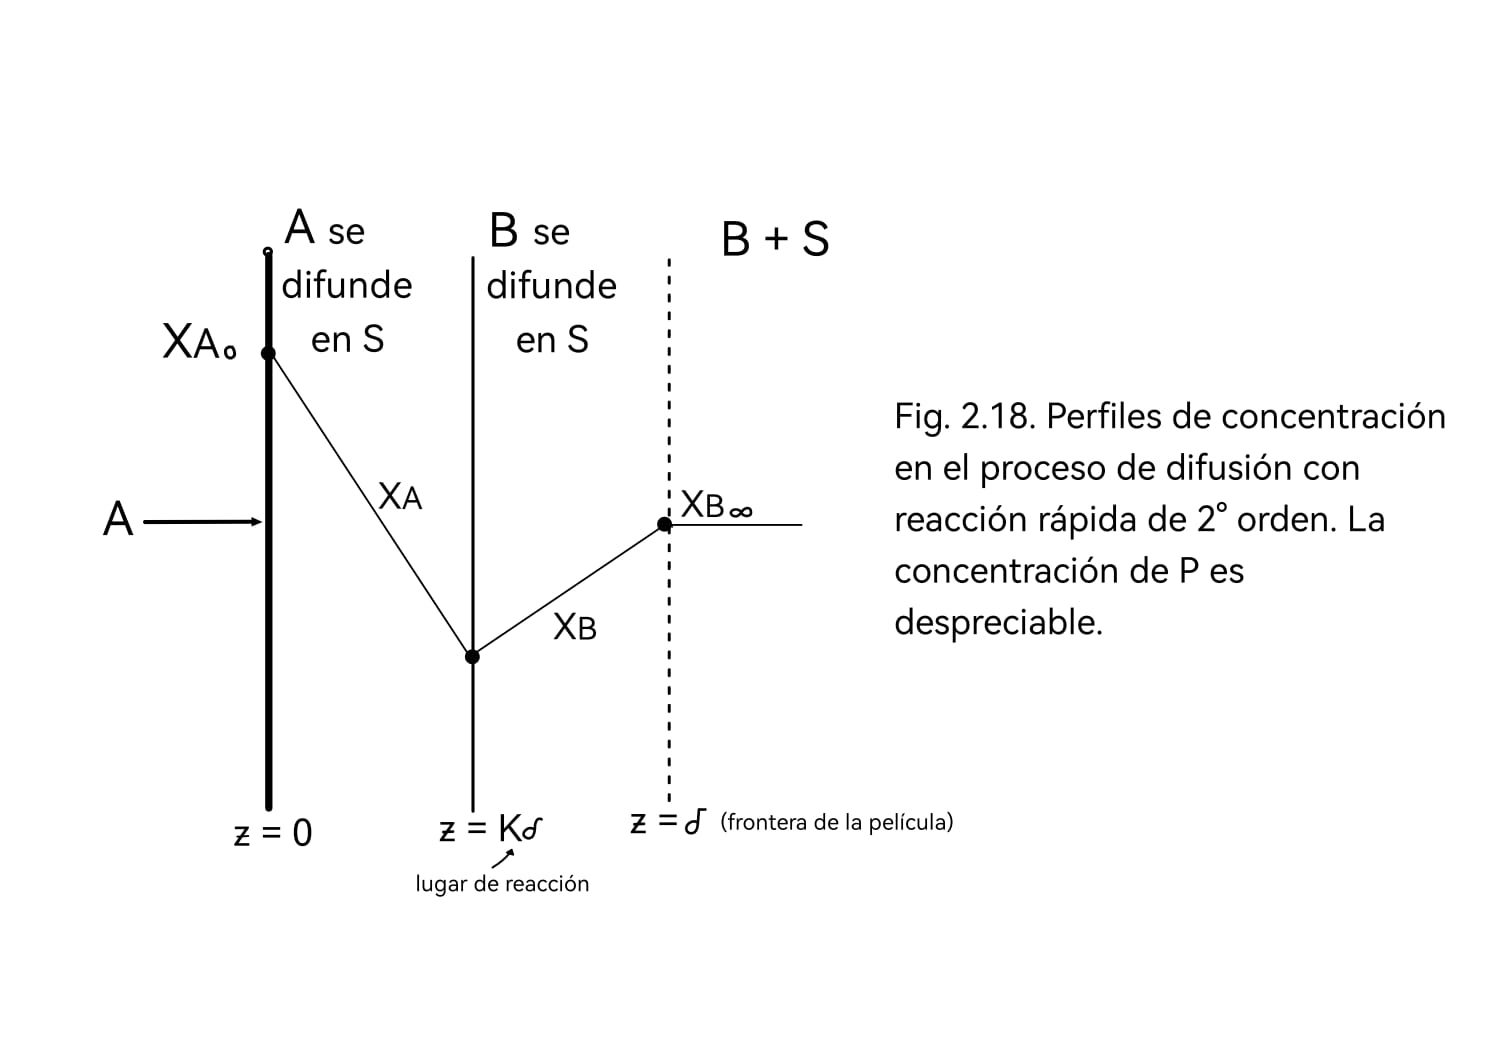
\includegraphics[width=0.5\textwidth]{imagen.8.jpg} 
    \label{fig:etiqueta}
\end{figure}
\flushleft
\textit{Respuesta:}
\flushleft
(a)-\quad $
N_{Az} \bigg|_{z= D}=\frac{cD_{AS}x_{A_D}}{\delta} 
$
\flushleft
(b)-\quad $
N_{A2} \bigg|_{z=D}=\frac{cD_{AS}x_{A_D}}{\delta}(1+\frac{x_{BD}D_{BS}}{x_{AD}D_{AS}})
$
\newpage
\textbf{3. Demanda de oxígeno por agregados de bacterias}\textit{(Problema 18.B.19. Bird et al.)}
\flushleft
Supongan un agrergado de bacterias esferico de R. Se desea determina la demanda de $O_2$ del agregado como función su tamaño, concetración de $O_2$ ($\rho_0$) en la superficie del agregado, la actividad metabólica de la células y el comportamientos difusinal del $O_2$. Supone que la difusión de $0_2$ está expresada como $r_{O_2}=-k_0$ y el comportamiento difusional esta gobernado por la ley de Fich condifusividad $D_{\upsilon_2m}$
\flushleft
(a)-Demostrar que el perfil de concentración de $O_2$ se describe por medio de la siguiente ecuación:
\[
\frac{1}{\xi^{2}}\frac{d}{d\xi}(\xi^{2}\frac{dx}{d\xi})= N \quad \text{donde} \quad X=\frac{\rho_{02}}{\rho_0},\quad  \xi=\frac{r}{R} \quad y \quad \nu= \frac{k_R^{2}}{\rho_0D_{O_2m}}
\]
(b)- Si $N$ es grande, tal que $x=0$ para $\xi<\xi_0$, existe zona central en el agregado sin $O_2$. Se reconoce que $X$ y $\frac{dX}{d\xi}$ son cero en $\xi=\xi_0$. ¿Cual es el significado físico de estos suposiciones?
\flushleft
(c)- Integrar la ecuación anterior con las condiciones de frontera propicios.
\flushleft
\textit{Respuesta:}
\[
x= 1 -\frac{N}{6}(1-\xi^{2})+\frac{N}{\xi}\xi^{2}_0(\frac{1}{\xi}-1) \quad  donde \quad \xi_0 \quad \text{es determinado por la siguiente ecuación:}\quad \xi^{3}_0-\frac{3}{2}\xi^{2}_0 +(\frac{1}{2}-\frac{3}{\xi})=0
\]
\newpage
\section*{Tarea 5}
\textbf{1. Difusión y reacción heterogenea en el tubo con un extremo cerrado.} \textit{(Problema. 18.B.15 Birt et al.)}
\flushleft
\begin{minipage}{0.4\textwidth} % Tamaño del bloque de la imagen
    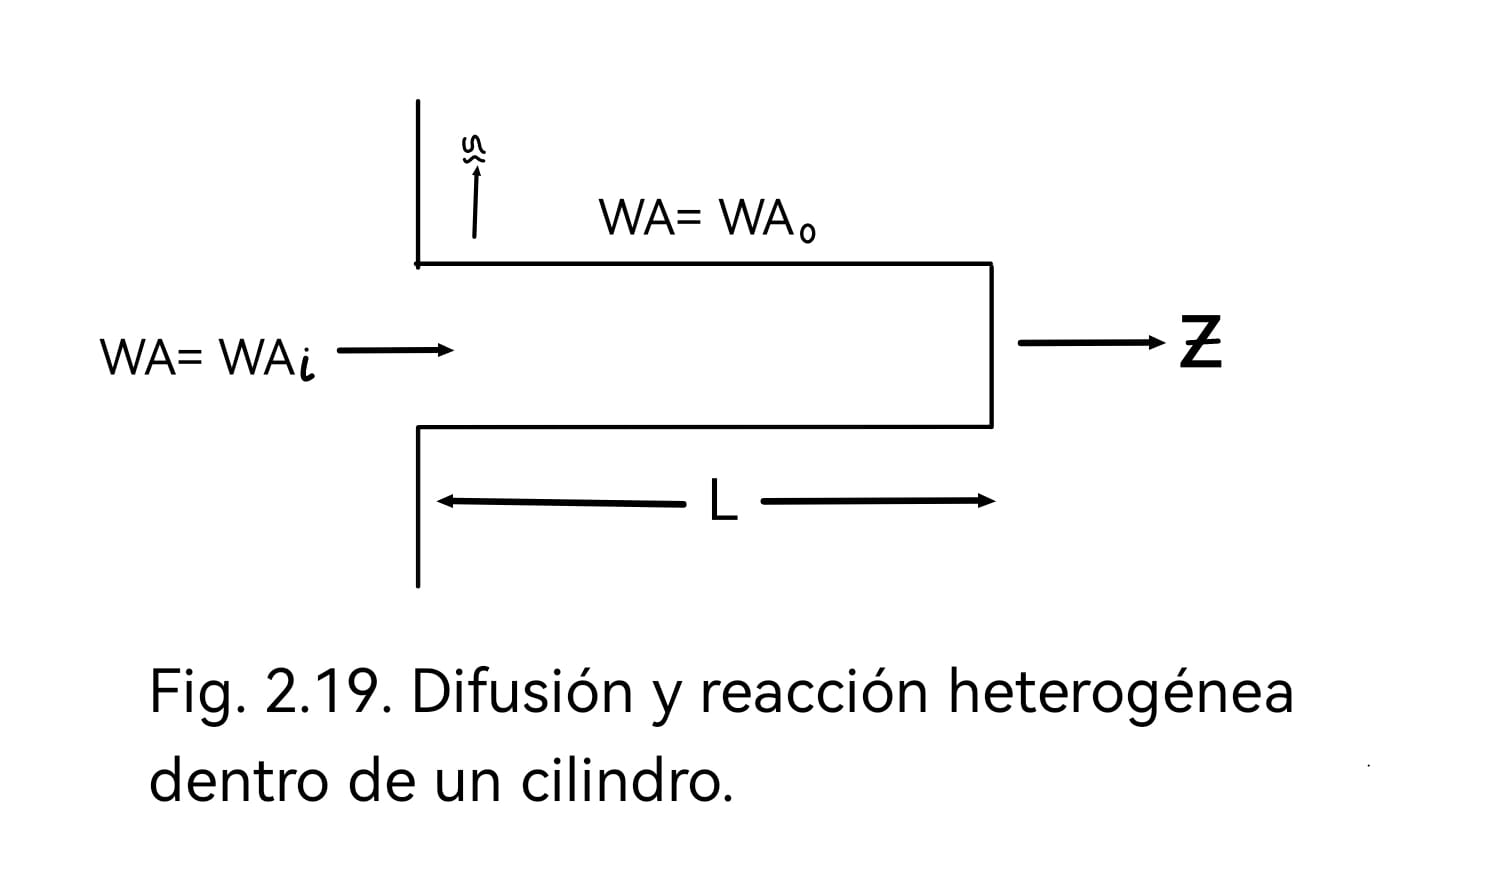
\includegraphics[width=\linewidth]{imagen.7.jpg} % Imagen ajustada al bloque
\end{minipage}
\hfill % Espaciado entre imagen y texto
\begin{minipage}{0.5\textwidth} % Tamaño del bloque del texto
Un poro cilíndrico de longitud \( L \) y sección \( S \) está en contacto con un fluido en su extremo abierto. El fluido contiene \( A \) y \( B \),  en donde \( A \) desaparece dentro del poro, se difunde a lo largo y reacciona sobre las paredes. El flux normal a la superficie es función de la fracción masa \( W_{AU} \) de \( A \) sobre la superficie y depende de \( z \). La temperatura y densidad son constantes, ya que la concentración de \( A \) es pequeña. Como el poro es largo, los gradientes de concentración normales a \( z \) son pequeños.
\end{minipage}
\flushleft
(a)-  Mostrar que el régimen es permanente.\quad
$
\frac{dWA}{dz} = \frac{P}{S} f(WA)
$
\flushleft
(b)- Demostrar que la velocidad promedio másica \( V_{z} \) es cero para este sistema.
\flushleft
(c)- Sustituir la ley de Fick \( J_A = -\rho D_{AB} \nabla WA \) en la ecuación anterior e integrar la expresión resultante para el caso \( f(WA) = k_iW_{A_0} \).  La condición de frontera en \( z = L \) supone que no hay reacción en ese extremo.
\flushleft
(d)- Desarrolla una expresión para \( W_A \) en el cilindro.
\flushleft
\textit{Respuesta:}
\flushleft
(c)- \quad$
    \frac{WA}{WA_i} = \frac{\cosh N \left[1 - \frac{z}{L}\right]}{\cosh N} \quad donde \quad N=\sqrt{\frac{PL^{2}k_1}{S{\rho}D_{AB}}}
    $
\flushleft
(d)- \quad$ W_A=(\frac{S{\rho}D_{AB}W_{Ai}}{L})N \tan{h}N $
\flushleft
\vspace{0.5cm} 
\textbf{2. Cálculo de la longitud de un reactor isotérmico.}\textit{(Problema 18.C.4 - Bird et al.)}
\flushleft
Sea \( a \) el área de la superficie de un catalizador y \( S \) la sección del reactor. Suponer que el flujo másico es \( w \) (en \(\text{lbm}/\text{hr}\)).
\flushleft
(a)- Mostrar que el balance a régimen permanente de \( A \) a una distancia \( L \) está dado por:
 \[
    \frac{dW_{A_0}}{dL} = - S a N A
    \]
(b)- Utilizar la ecuación (2.74) y el resultado anterior para obtener una expresión de la longitud \( L \) necesaria para convertir la composición a la entrada \( X_A(0) \) en la de la salida \( X_A(L) \). Utilizar la relación:\quad
    $
    \gamma_\alpha = M_\alpha N_\alpha
    $
\flushleft
\textit{Respuesta:}
  \[
    L = \frac{w \delta M_B}{25 a cD_{AB}} \int_{X_A(0)}^{X_A(L)} \frac{dX_{A_0}}{\left[ {M_A X_{A_0} + M_B (1 - X_{A_0})} \right]^2 \ln \left( 1 - \frac{1}{2} X_{A_0} \right)}
    \]
\flushleft
\vspace{0.5cm} 
\textbf{3. Difusión y reacción química en un líquido}\textit{(Problema 19.B.6 - Bird et al.)}
\flushleft
(a)- Una esfera sólida de \( A \) está suspendida en un líquido \( B \) en el que \( A \) es ligeramente soluble y en donde \( A \) reacciona con constante cinética. Mostrar que el perfil de concentraciones es:
\[
    \frac{C_A}{C_{A_s}} = \frac{R}{r} \frac{e^{-b\frac{r}{R}}}{e^{-b}}, \quad b^2 = \frac{k_1R^{2}}{D_{AB}}
    \]
 \( R \) es el radio de la esfera y \( C_{A_s} \) es la solubilidad molar de \( A \) en \( B \).
 \flushleft
 (b)-  En régimen cuasiestático, calcular la disminución del diámetro de la esfera a medida que se disuelve y reacciona.  Mostrar que la relación radio/ tiempo en: 
   \[
    \sqrt{\frac{k_1}{D_{AB}}} (R - R_0) - \ln \frac{1 + \sqrt{\frac{k_1}{D_{AB}}} R}{1 + \sqrt{\frac{P_B}{D_{AB}}} R_0} = -\frac{k_1 C_{A_0} M_A (t - t_0)}{\rho_s}
    \]
en donde \( R_0 \) es el radio de la esfera en \( t_0 \) y \( \rho_s \) es la densidad de la esfera.
\newpage
\section*{Tarea C}

\textbf{1. Factor de efectividad en discos delgados} \textit{(Problema 18.B.14 - Bird et al.)}
\flushleft
\begin{minipage}{0.4\textwidth} % Tamaño del bloque de la imagen
    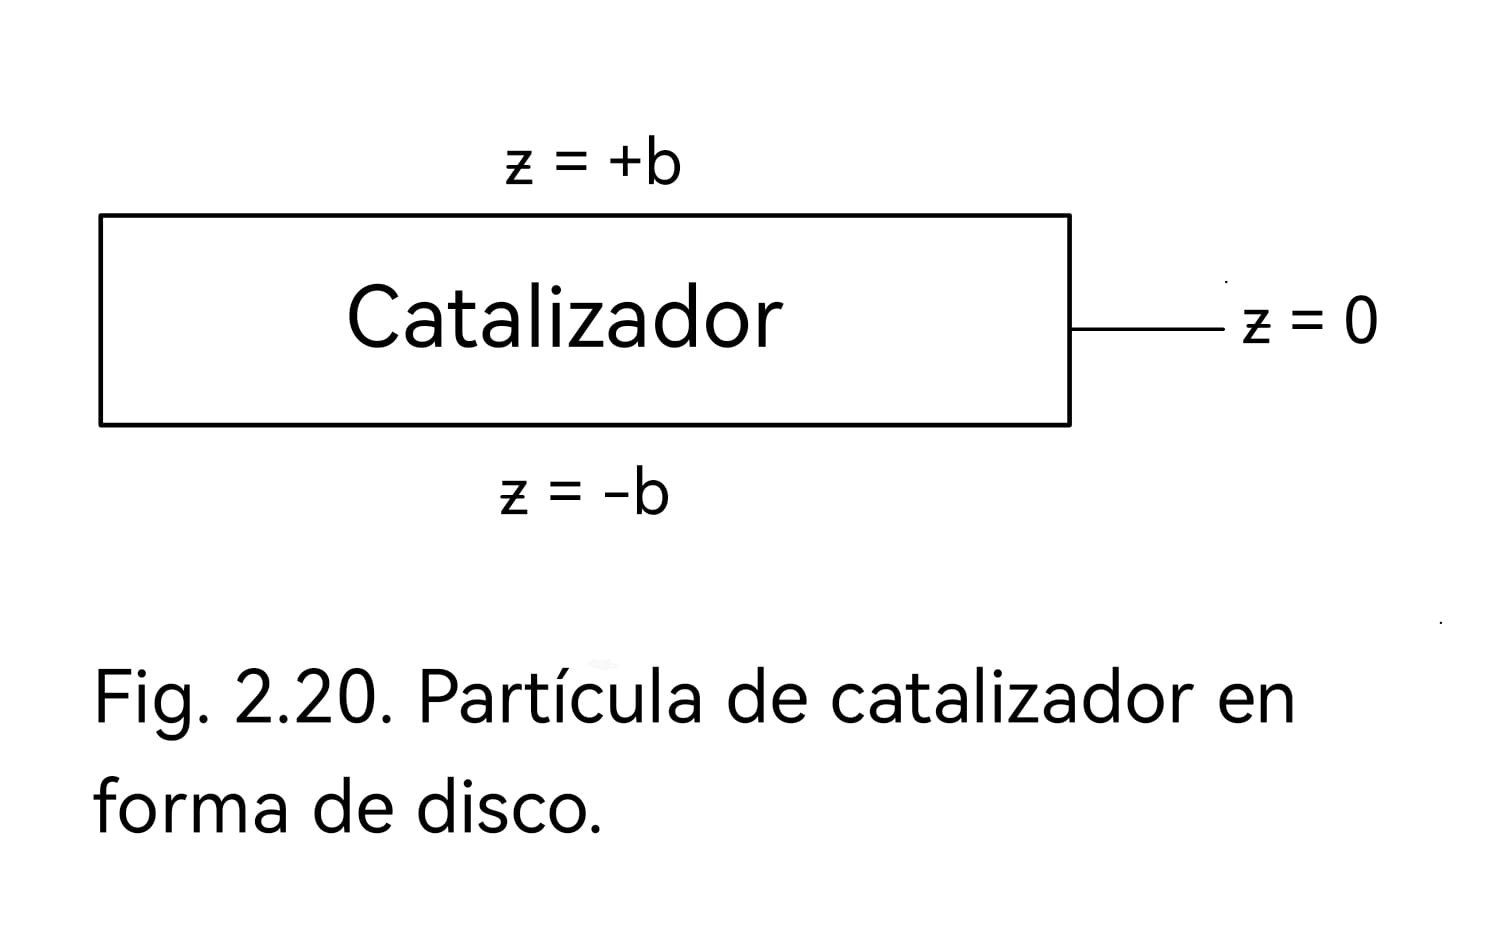
\includegraphics[width=\linewidth]{imagen.5.jpg} % Imagen ajustada al bloque
\end{minipage}
\hfill % Espaciado entre imagen y texto
\begin{minipage}{0.55\textwidth} % Tamaño del bloque del texto
Considerar en este caso que el área del grosor del disco es muy pequeña en comparación con el área de los discos. Demostrar que el perfil de concentraciones es:
\end{minipage}
\[
 \frac{C_A}{C_{A_s}} = \frac{\cosh \left(\frac{\lambda}{D_{AB}} z\right)}{\cosh \left(\frac{\lambda}{D_{AB}} b\right)}
    \]
Mostrar que el flujo másico en las superficies \( z = \pm b \)  es:
\[
    |W_A| = 2 \pi R^2 C_{A_s} D_{AB} \lambda \tanh \lambda b, \quad \lambda=\sqrt{\frac{k_1a}{D_A}}
\]

Mostrar que si el disco es cortado paralelo al plano \( x-y \) en varios  cortes o rebanadas $n$, el flujo másico total sería:
\[
    |WA^{(n)}| = 2 \pi R^2 C_{A_s} D_{AB} \lambda n \tanh \left(\frac{\lambda b}{n}\right)
    \]
Obtener la expresión del factor de efectividad tomando el límite:
    \[
    \eta_A = \lim_{n \to \infty} \frac{|WA|}{|WA^{(n)}|} = \frac{\tanh (\lambda b)}{\lambda b}
    \]
    











